\documentclass[a4paper, 12pt]{article}
\usepackage{wrapfig}
\usepackage{float}
\usepackage{graphicx}
\usepackage{cite}
\usepackage{hyperref}
\usepackage{enumerate}
\author{Ryan J. Kinnear - 200273748 \\ Raza Rauf}
\title{ENEL 400 - Software Radio Design}
\date{\today}

\begin{document}
\maketitle

\section{Background}
A software defined radio (SDR) is essentially a digital radio.  An analog front end device such as a DVB-T USB Dongle \cite{usb_dongle}, HackRF \cite{hackrf}, or the USRP \cite{usrp} receives and digitizes a radio frequency signal and sends the samples to a computer.  The ideal software defined radio consists of an analog to digital converter with one end connected directly to an antenna, and the other end connected to a computer.  A realistic implementation requires a significant analog component to digitize RF signals, as well as significant preprocessing on the digital signal (usually accomplished by an FPGA).

A complete SDR consists of an analog digitizing front end, and a large software system.  The point of this architecture is to achieve flexibility.  If the demodulator (ie. FM demodulator, QAM demodulator, PSK demodulator ...) is implemented in hardware as in a traditional radio, the receiver is only capable of extracting information (bits, or an baseband analog waveform) from a certain type of signal.  For example, an FM radio receiver can't receive a 64QAM signal.  If the demodulator is implemented in software, the effort required to redesign to demodulate a new type of signal is reduced substantially.  Examples of SDR software are GNURadio \cite{gnu_radio} or SDR\# \cite{sdr_sharp}.  A software package needs to be integrated with a compatible RF front end.

The scope of our ENEL400/ENEL417 project is to implement the hardware front end, and a simple processing algorithm in an FPGA to demodulate broadcast FM radio.  Ideally, the system should be capable of sending samples to a computer, simply into a text file.  There are no plans to integrate our hardware with either a full software radio suite, or any of our own real time processing software.  Although we may be able to write a (non real-time) demodulator that acts on a plain file, time permitting.

\section{RF Front End Design}

\begin{figure}
\caption{System Diagram}
\label{fig:system_diagram}
\centerline{\includegraphics[width=15cm]{system_diagram.jpg}}
\end{figure}

Figure \ref{fig:system_diagram} is the design for the RF front end.  The FPGA element will be presented in the next section.  The items in the system diagram are numbered in orange to help the reader follow what is being referred to.

An antenna (1) is fed into a MAX3543 (6) television tuner/receiver.  This chip handles the main RF processing.  It filters out an \~8MHz band (primarily through the IF filter (7) which will be either a SAW filter or a LC ladder), anywhere between roughly 60MHz to 800MHz.  See figure \ref{fig:transfer_function}.  This is then downconverted to an apparently standard centre frequency of 36MHz.  The output is an analog differential signal.  This differential signal is fed into a fully differential operational amplifier (an ADC driver), and into the analog to digital converter.  The ADC is controlled by the FPGA.  Digital data is shifted 12 parallel bits at a time to the FPGA through an FPGA Mezzanine card (FMC \cite{fmc}).  This connector is conveniently present on the FPGA boards provided in the lab.

The MAX chip requires an I$^2$C interface to control various parameters such as the gain and the centre frequency of the RF filter.  This will be controlled by either the STM32 microcontroller, or a beaglebone black.  This is probably far easier than using the FPGA.  However, it should be easy to also connect the I$^2$C control line to the FPGA through the FMC, in case we find a use for it..

Finally, a digital stream of data (likely 12b wide, although I have for some reason written 8b on the diagram) will be shifted out of the FPGA into a DAC, into a driver, and then a simple speaker.

Ideally, the FPGA will have an Ethernet, USB, or Uart output to send data directly to a computer.

\begin{wrapfigure}{L}{0.60\textwidth}
\caption{MAX3543 Transfer Function}
\label{fig:transfer_function}
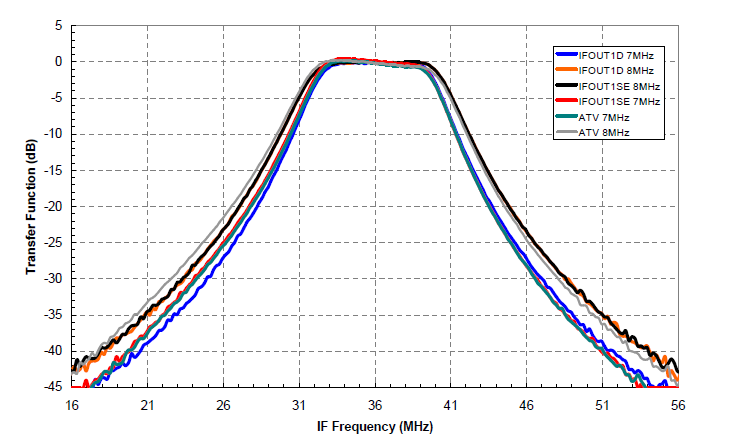
\includegraphics[width=9cm]{../../../transfer_function.png}
\end{wrapfigure}

\section{Test Summary}

Each labelled component is listed and a quick summary of the test plan is provided here.  The next section is a longer description.  Most of the test procedures pertain to the testing that will be done after a PCB has been fabricated.  Most of the system design, and a lot of the detailed design is done.  There should be time to fabricate a second PCB if the first one fails.  A lot of the challenge with this project is that many components are hard or impossible to test without a printed circuit board.  Because of this, I have designed and am in the process of having fabricated a test PCB for one of the critical components.  A SPICE model for the ADC is also planned, see the following section.  A Python model of the basic demodulation algorithm has been implemented, I have not included this here but would be available upon request.  This model verifies that our overall system plan should be feasible.

\begin{enumerate}
  \item (antenna) Test with spectrum analyzer. %1
  \item (Diplex filter) No test needed. %2
  \item (120V adapter) No test needed. %3
  \item (3.3V regulator) Test on breadboard.  Probe connections with DMM.  Measure output with DMM. %4
  \item (3.0V regulator) Probe connections with DMM.  Measure output with DMM. %5
  \item (MAX3543 radio tuner) Control with STM32 or BeagleBone.  Measure inputs/outputs with scope.%6
  \item (IF filter) PCB test board to be fabricated. %7
  \item (ADC Driver) Probe connections with DMM.  Minimal test necessary. %8
  \item (Anti Aliasing Filter) PCB test board to be fabricated. %9
  \item (ADC) Dev board for similar part. %10
  \item (FMC connector) Probe connections with DMM. %11
  \item (DAC) Probe connections with DMM.  If it fails, the STM32 is a backup. %12
  \item (I$^2$C) This is a test connector. %13
\end{enumerate}

\section{Hardware Test/Checkout Plan}
The first part of the system is an antenna, labelled (1).  This antenna should be a 75 $\Omega$ antenna that is sensitive to FM broadcast frequencies (\~100MHz).  I had a 50 $\Omega$ antenna already, and have tested the return loss of it in the lab with a spectrum analyzer.  The results are summarized in my log book.  My findings are that the antenna is very bad.  The return loss is very high in the frequencies of interest, and I was unable to see any FM stations at all inside the lab.  It may work outdoors however, as I was unable to receive FM using my DVB-T dongle inside the lab either.  This antenna can be easily replaced with a standard 75 $\Omega$ TV antenna, which should be more than adequate.

Item (2) in the diagram is a 120V AC/DC adapter.  This is straightforward, any 9V adapter will do.  The power requirements will be very low.

Item (3) is a diplexer.  This is an RF filter which splits the spectrum into very high frequency (VHF) and ultra high frequency (UHF).  The reason for this is simply that the MAX3543 (6) requires it.  I do not need to design this filter, it is specified (even the PCB layout) by the manufacturer.  As such I am mostly assuming it will work as desired.  I will not perform any testing other than what testing I can do with a multimeter on the pads of the PCB.

(4) is a 3.3V regulator.  The current plan is to use an LT1086 \cite{lt1086}, but this is not finalized.  The test plan will be to wire the device into a breadboard and read the output with a digital multimeter.  The PCB can also be probed with a digital multimeter to ensure connectivity between the regulator output pad and all of the power pin pads for each component on the board.  There will likely not be any power planes on the PCB as MAXIM has strongly recommended using a 2 layer board.  The reason is that a few inductors placed close to the MAX chip have a highly specific layout that has been optimized by a computer, this will effected by a 4 layer board (most of their customers at the time were using 2 layer boards, so that is what they designed for).  I may disregard this recommendation if placing and routing all the components on a 2 layer board proves to be too difficult.  However, it remains an option to route to less critical components via jumper wires.

The ADC and the ADC driver both require 3V supplies.  So, (5) is a 3.0V regulator.  It will be tested in a similar fashion on the 3.3V regulator.  Note that it will be important to ensure that the 3V and the 3.3V regulators are not shorted together.  The power supplies will be the first things soldered to the board, as they are easy to test, and are required for the operation of mostly everything else.

Number (6) is the MAX3543 chip that has been described in the System Design section.  This is the most complex component of the system as well as the most difficult to test.  It needs to be configured via an I$^2$C interface, which will be provided by the STM32, at least for testing purposes.  Fortunately, the frequency that is expected to be output from the MAX3543 are well within the bandwidth of the scopes in the lab.  It will not be necessary to design in any RF connectors for the spectrum analyzer.  There is also a recommended layout for this chip and it's supporting circuitry provided by Maxim.  This layout will be followed as closely as possible.

The IF filter (7) is also an important component of the design.  A large portion of the RF filtering is performed outside the MAX chip in this IF filter stage.  I have been provided a number of surface acoustic wave (SAW) filters by Golledge \cite{golledge}.  These filters have the required specifications, however I am unsure about how they will actually perform.  I am also quite confused about impedance matching.  The lengths of my tracks are far below even a 10th of the wavelength of a 36MHz signal propagating through FR4, so I don't think impedance matching will come into play.  At the time of writing (Nov 25th/2014) I have designed a test PCB for an LC anti-aliasing filter and the SAW filter (figure \ref{fig:test_pcb}.  This test circuit will settle my confusion.  If the SAW filter performs poorly, I will be able to replace the IF filter (7) easily with an LC ladder filter.

\begin{figure}[h]
\caption{IF Filter Test PCB}
\label{fig:test_pcb}
\centerline{\includegraphics[width=11cm]{test_pcb.png}}
\end{figure}

Item (8) is an AD8138 differential op-amp.  It is recommended for driving the AD9235 for anything below \~100MHz.  For optimal performance analog devices actually recommends a higher performance amplifier, but the higher end amplifiers are absolutely minuscule (difficult to solder), and operate at a different voltage.  These drawbacks are enough to decide the AD8138 is satisfactory.  There isn't much of a test plan for this device, it is a very simple component, has excellent documentation and app-notes, and only comes in surface mount packages.

Number (9) is an anti-aliasing filter.  I have designed this filter using the Genesys \cite{genesys} software package, and will be present on the PCB test board along with the SAW filter.

The ADC (10) will be an AD9235 \cite{ad9235}.  This component is the interface between the RF front end (my section) and the FPGA (Raza's section).  Dr. Zhang has provided us with a test board for a different ADC.  Raza plans to build an ADC controller (in the FPGA) using this board.  We expect the process to be very similar, and that a controller for the test board will work with the AD9235 with only minor modifications.  This is another component where I am confused about impedance matching, I don't know if I need to worry about it.  I suspect it is not an issue as there is not really any information about it in the datasheet.  But, Dr. Zhang has suggested I test the device using SPICE.  Unfortunately Analog Devices does not provide a SPICE model for this part, but I will hopefully be able to create a satisfactory model by looking at other ADC models.

\begin{wrapfigure}{R}{0.8\textwidth}
\caption{FMC Connector - http://danstrother.com/2010/12/04/fmc-lpc-to-sata-adapter-board/}
\label{fig:fmc_conn}
\includegraphics[width=8cm]{fmc_conn.jpg}
\end{wrapfigure}

The connector (11) between the ADC and the FPGA is a standard FPGA mezzanine connector \cite{fmc}.  See figure \ref{fig:fmc_conn}  This is a simple passive connector, the female side is conveniently on the FPGA board from the lab.  As long as I route everything to the correct pins, this connector should not pose any problems.

The output DAC (12) is an as yet unspecified digital to analog converter.  Alternatively, we could use the DAC on the STM32 board.  This will be designed to output demodulated FM signals.  It is undrawn, but the connection to the speaker probably requires some kind of driver.

Item (13) are a set of pins to connect control signals to the STM32 board.  These are passive pins, the only problem may be routing to them through a 2 layer board.  However, as with some power lines, these are not critical or high speed signals.  It may be possible to connect things through long jumpers.

(14) is the STM discovery board, or possibly a Beagle Bone Black \cite{bbb}.  The purpose of this will be to control the tuning and gain of the MAX3543.  I plan to connector the I$^2$C to the FPGA as well through a jumper.  It is just expected that it will be far easier to control everything with the micro controller rather than the FPGA.  Programming the STM32 is straightforward, and it has an on board I$^2$C controller.  Alternatively, I could replace the STM32 with the BeagleBone Black and interface the pins with a Python script.  This interface can be checked and debugged using the trigger feature of the oscilloscope.  A logic analyzer would also work, but I have never actually used one before.

\section{Additional Concerns}

\begin{wrapfigure}{L}{0.5\textwidth}
\caption{MAX3543}
\label{fig:qfn40}
\centerline{\includegraphics[width=5cm]{QFN40.jpg}}
\end{wrapfigure}

\underline{Soldering} is a concern.  The MAX3543 (see figure \ref{fig:qfn40}) and the FMC connector (figure \ref{fig:fmc_conn}) will both be difficult to solder.  The MAX3543 is a 6x6mm 40pin QFN chip, I really did not appreciate how small this actually was until I saw it in person.  I have seen a number of YouTube videos of people soldering these and it does not seem like it is beyond our capability.  Tin the pads, use a heat gun, a lot of flux, and the chip falls into place on the pads.  The FMC connector will also pose a problem.  Dr. Zhang has said this is really the best connector for us.  I have read that using solder paste and a toaster oven or hotplate should work for this connector.

\underline{Gain Control}.  The MAX3543 should output a constant amplitude signal from it's differential output, however there is still a pin for IF gain.  It is stated in the datasheet that ``The MAX3543 is designed to control it's own RF gain ...'' however it is unclear how much AGC is provided by the MAX chip itself. It may be necessary to control the gain ourselves.  This can be accomplished by a micro controller or a knob. 

\clearpage
\bibliography{../refs/fourth_year.bib}
\bibliographystyle{plain}
\end{document}